\chapter{Grundlagen}
\label{chap:grundlagen}
    In diesem Kapitel werden die für diese Thesis relevanten Grundlagen geschaffen, um ein Grundverständnis und 
    fundiertes Wissen über verwendete Technologien zu erlangen und die nachfolgende Recherche, Konzeption und 
    Umsetzung besser verstehen zu können. 

\section{Internet der Dinge}
\label{sec:iot}
    Das \ac{IdD}, im Englischen \ac{IoT}, zählt als eines der Schlagworte in der \ac{IT}. In der Domäne des \acs{IoT} bekommen 
    Gegenstände und Objekte eine eindeutige Identität, die eine Kommunikation miteinander als auch das Entgegennehmen von 
    Befehlen erlaubt. Mit dem \acl{IdD} lassen sich Anwendungen sowie Prozesse automatisieren und Aufgaben erledigen ohne das 
    von außen Eingegriffen werden muss \cite{bigdatainsider2016}. Die Prozessautomatisierung findet sich auch im Kontext des 
    \acl{SH} wieder, welches in nachfolgendem Kapitel genauer aufgegriffen wird. 
    \\
    \linebreak
    In der einschlägigen Literatur gibt es für das \acl{IoT} keine allgemeingültige Definition die alle Anwendungsbereiche abdeckt. 
    Die Definitionen und Auslegungen der Interpretation unterscheiden sich je nach Anwendungsgebiet. Demnach gibt es viele verschiedene 
    Forschungsgruppen, darunter Forscher, Akademiker, Innovatoren, Entwickler und Geschäftsleute, die den Begriff oder die zugrundeliegende 
    Problemstellung definiert haben. Die Ursprünge jedoch sind dem Experten für digitale Innovationen, 
    Kevin Ashton\footnote{Britischer Technologie-Pionier, Mitgründer des Auto-ID Centers am Massachusetts Institute of Technology (MIT). \url{https://de.wikipedia.org/wiki/Kevin_Ashton} (Abgerufen am 22.03.2022)}, 
    zuzuschreiben. 
    \\ 
    Die in der Literatur auffindbaren Definitionen verfolgen zwei Sichtweisen, zum Einen aus Sicht des aktiven, dass die Daten von 
    Menschen erstellt wurde, zum Andere, aus Sicht des passiven, dass die Daten von Dingen, darunter die Sensoren und Aktoren, 
    erstellt wurde. \cite{Madakam2015} Eine aus dem Zusammenschluss hervorgehende Definition ist, dem wissenschaftlichen Artikel zufolge, folgende:
    % „Ein offenes und umfassendes Netzwerk intelligenter Objekte, die in der Lage sind, sich automatisch zu organisieren, 
    % Informationen, Daten und Ressourcen auszutauschen und auf Situationen und Veränderungen in der Umgebung zu reagieren 
    % und zu handeln.“
    \pagebreak
    \begin{quote}
        “An open and comprehensive network of intelligent objects that have the capacity to auto-organize, share information, data 
        and resources, reacting and acting in face of situations and changes in the environment” \cite{Madakam2015}
    \end{quote}
    Daraus kann die Ableitung erfolgen, dass der Begriff des \acl{IdD} für die Vernetzung von Gegenständen im privaten Gebrauch oder 
    von Geräten und Maschinen im industriellen Umfeld über das Internet steht. Damit Geräte individuell angesprochen werden können, werden diese 
    mit einer eindeutigen Identität, genauer einer \ac{IP}-Adresse, im Netzwerk belegt und mit elektronischer Intelligenz ausgestattet \cite{bigdatainsider2016}.
    Darüber sind die Netzwerkteilnehmer im Stande, über das Internet zu kommunizieren Prozesse automatisiert zu erledigen. Die sogenannten 
    \textit{intelligenten Geräte} werden auch oft mit dem englischen Begriff, \textit{Smart Devices}, betitelt. 
    \\
    \linebreak
    Neben der Kommunikation der Geräte über das Netzwerk untereinander kann ebenso entweder durch das Gerät selbst oder eine zentrale 
    Schnittstelle über das Internet interagiert werden. Dadurch sind Objekte und Gegenstände durch einen Benutzer von beliebigen Orten 
    auch außerhalb des Netzwerks erreichbar und können so bedient werden. Diese Art und Weise wird auch in dem zentralen Thema des 
    \acl{SH} verwendet. Die Funktion als auch die Umsetzung wird im Kapitel (\ref{sec:smartHome}) näher beleuchtet.
    \\
    \linebreak
    Das \acl{IdD} ist ein nahezu existenzielles Konzept der \acs{IT}-Welt. Mit dem \acs{IoT} wird die Vision verfolgt eine globale 
    Infrastruktur zu erstellen, mit dem physische Objekte miteinander vernetzt werden und jeder Zeit zur Verfügung stehen. Das \acl{IoT} 
    kann auch als globales Netzwerk angesehen werden, indem die Kommunikation zwischen Mensch zu Mensch, Gerät zu Mensch und Gerät zu 
    Gerät ermöglicht. In vielen Artikeln wird auch davon gesprochen, dass mit der Technologie die Verschmelzung der digitalen und 
    der physischen Welt vorangetrieben wird.\footnote{Das Internet der Dinge – der digitale Zwilling der Welt. Kompetenzzentrum Öffentliche IT in Kooperation mit dem Fraunhofer Institut. \url{https://www.oeffentliche-it.de/trendsonar-iot} Abgerufen am 23.03.2022.} 
    Die Vereinigung beider Welten ist die Verknüpfung physischer Objekte, die eindeutig identifizierbar sind, mit einer virtuellen 
    Repräsentation in einer vergleichbaren Internet-Struktur. 

    \subsection*{Gesamtbild des \acl{IoT}}
        Der folgenden Abbildung (\ref{pic:mindmap_IoT}) ist zu entnehmen, welche Technologien rund um das \acl{IdD} liegen und in Verbindung damit stehen. 
        \begin{figure}[hbt!]
            \centering
            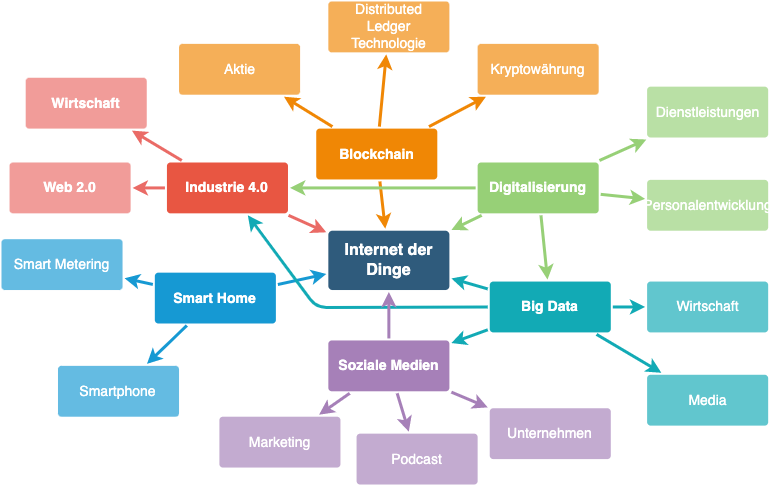
\includegraphics[width=13cm,height=13cm,keepaspectratio]{images/IoT-Mind_Map.png}
            \caption{Technologische Einordnung von IoT \cite{iotmindmap2018}}
            \label{pic:mindmap_IoT}
        \end{figure}
        \\
        \linebreak
        %\pagebreak
        Beispielsweise ist das \acs{IoT} eine wesentliche Grundlage für das Themengebiet \textit{Big Data}. Die durch Sensoren und Aktoren erzeugten Daten 
        können Grundlage für die Verwendung im Bereich \textit{Big Data} sein. Dabei werden die Datenmengen gespeichert und mithilfe von Mustern 
        und Herangehensweisen des Big Data\footnote{Definition und Funktionsweise von Big Data. \url{https://www.oracle.com/big-data/what-is-big-data/} Abgerufen am 25.03.2022} analysiert. 
        Big Data ist kein Bestandteil dieser Arbeit und wird demnach nicht weiter ausgeführt. Das Beispiel dient lediglich zu Veranschaulichung 
        und Interpretation der oben aufgeführten Abbildung (\ref{pic:mindmap_IoT}).
        \\
        \linebreak
        Eine allgemeine exemplarische Skizzierung eines Systems, welches nach dem \acs{IoT}-Konzept aufgebaut ist, kann der folgenden 
        Abbildung (\ref{pic:skizze_iot}) entnommen werden:
        \begin{figure}[hbt!]
            \centering
            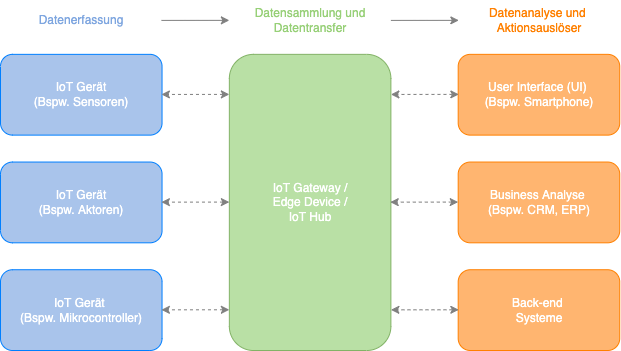
\includegraphics[width=13cm,height=13cm,keepaspectratio]{images/IoT_Grundstruktur.png}
            \caption{Exemplarische Darstellung eines \acs{IoT}-Systems \cite{iotskizze2022}}
            \label{pic:skizze_iot}
        \end{figure}
        Hierbei werden die jeweiligen Komponenten verdeutlicht, die in einem System zu finden sind. Mit den \textit{IoT-Geräten}, darunter 
        beispielsweise Sensoren und Aktoren, findet die Datenerzeugung statt. Mit dem dahinterstehenden \textit{Gateway} werden die aus den Geräten 
        erzeugten Daten gesammelt und an zentraler Stelle an die Cloud gesendet, in der danach eine Analyse auf die erzeugten Daten 
        durchgeführt werden kann.

    \subsubsection*{Anwendungsbereiche des \acs{IoT}}
        Grundlegend können im Bereich des \acl{IoT} zwischen zwei Anwendungsbereichen unterschieden werden, zum Einen im privaten Bereich und zum 
        Anderen im industriellen Bereich. Der private Bereich deckt hauptsächlich die Thematik rund um den Gebrauch von Alltagsgegenständen ab und 
        deren Vernetzung untereinander, um eine komfortablere und intelligentere Nutzung der Geräte zu ermöglichen. Darin inbegriffen sind 
        Gebäudeautomatisierungen und die Ereignissteuerung über das Internet. Diese Funktionen sind Hauptbestandteil des \acl{SH}-Konzeptes, welches 
        in Abschnitt (\ref{sec:aufbau}) genauer aufgegriffen wird. 
        \\
        \linebreak
        Der industrielle Bereich beschäftigt sich damit, Maschinen und Anlagen so miteinander zu vernetzen, dass sich ganze industrielle Prozesse 
        automatisiert lassen und so die Effizienz der Prozess- und Produktionsabläufe steigern. Die Nutzung des \acs{IoT} im industriellen Bezug 
        ist ein elementarer Bestandteil der heutigen \textit{Industrie 4.0}\footnote{Definition und Beschreibung der Industrie 4.0 \url{https://www.plattform-i40.de/IP/Navigation/EN/Industrie40/WhatIsIndustrie40/what-is-industrie40.html} Abgerufen am 25.03.2022}.
        Eine genauere Benennung dieser Sparte ist oft auch unter dem \textit{\ac{IIoT}} bekannt. An dieser Stelle wird zwischen den beiden Anwendungsbereichen 
        stark differenziert, da im Rahmen dieser Arbeit lediglich der Fokus auf dem privaten Bereich des \acs{IoT} liegt. 
        \\
        \linebreak
        Mit dem \acl{IdD}-Ansatz gibt es zwei Paradigmen, die in Kombination als auch separiert Anwendung finden. Diese werden in folgendem Abschnitt kurz erläutert.

        \subsubsection*{Edge und Cloud Computing}
            Bei den beiden Paradigmen handelt es sich zum Einen um Edge Computing und zum Anderen um Cloud Computing.
            \\
            Das Edge Computing verfolgt einen \textit{dezentralen Ansatz}, bei dem die Berechnung und Haltung der Daten näher bei der Datenerzeugung gehalten wird. 
            Dies bedeutet, dass jedes Gerät über eine eigene Intelligenz verfügt, bei der Daten direkt nach der Erzeugung verarbeitet und gespeichert werden können. 
            Zu späterem Zeitpunkt kann in From einer Datenbündelung oder einer Vorauswahl die Informationen an ein Rechenzentrum weitergegeben werden. 
            \begin{quote}
                “Edge computing is different from traditional cloud comput- ing. It is a new computing paradigm that performs computing at the edge 
                of the network. Its core idea is to make computing closer to the source of the data [...]” \cite{Cao2020}
            \end{quote}
            %Definition Cloud Computing (write 2-3 sentence)
            \begin{quote}
                “Cloud computing is a model for enabling ubiquitous, convenient, on-demand network access to a shared pool of configurable 
                computing resources (e.g., networks, servers, storage, applications, and services) that can be rapidly provisioned and 
                released with minimal management effort or service provider interaction.” \cite{Mell2011}
            \end{quote}
            %Unterschiede der beiden Ansätze und in Zusammenhang mit IoT (kurz)
    
    \subsection{Kommunikationsmodelle und Architekturen}
    % \cite{IEEE2015} http://www.informatik.uni-oldenburg.de/~iug18/iot/was_ist_IoT.html 

    \subsection{Historische Entwicklung}

    \subsection{Ziele von \acs{IoT}}
    \label{subsec:ziele-iot}
